% Created by tikzDevice version 0.12.3 on 2020-04-05 20:01:22
% !TEX encoding = UTF-8 Unicode
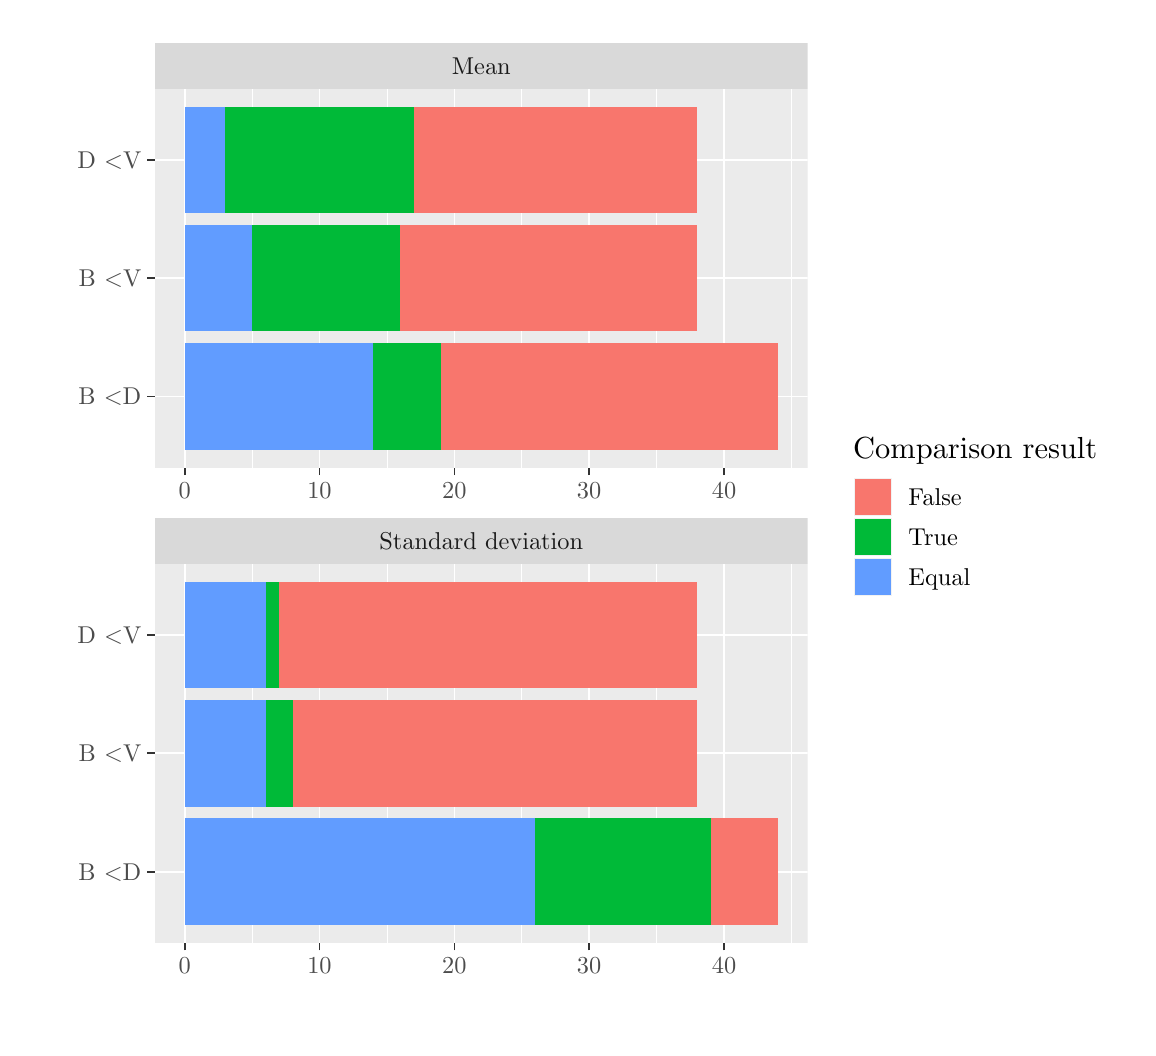
\begin{tikzpicture}[x=1pt,y=1pt]
\definecolor{fillColor}{RGB}{255,255,255}
\path[use as bounding box,fill=fillColor,fill opacity=0.00] (0,0) rectangle (397.48,361.35);
\begin{scope}
\path[clip] (  0.00,  0.00) rectangle (397.48,361.35);
\definecolor{drawColor}{RGB}{255,255,255}
\definecolor{fillColor}{RGB}{255,255,255}

\path[draw=drawColor,line width= 0.6pt,line join=round,line cap=round,fill=fillColor] (  0.00,  0.00) rectangle (397.48,361.35);
\end{scope}
\begin{scope}
\path[clip] ( 46.01,202.38) rectangle (281.82,339.28);
\definecolor{fillColor}{gray}{0.92}

\path[fill=fillColor] ( 46.01,202.38) rectangle (281.82,339.28);
\definecolor{drawColor}{RGB}{255,255,255}

\path[draw=drawColor,line width= 0.3pt,line join=round] ( 81.09,202.38) --
	( 81.09,339.28);

\path[draw=drawColor,line width= 0.3pt,line join=round] (129.81,202.38) --
	(129.81,339.28);

\path[draw=drawColor,line width= 0.3pt,line join=round] (178.53,202.38) --
	(178.53,339.28);

\path[draw=drawColor,line width= 0.3pt,line join=round] (227.25,202.38) --
	(227.25,339.28);

\path[draw=drawColor,line width= 0.3pt,line join=round] (275.98,202.38) --
	(275.98,339.28);

\path[draw=drawColor,line width= 0.6pt,line join=round] ( 46.01,228.05) --
	(281.82,228.05);

\path[draw=drawColor,line width= 0.6pt,line join=round] ( 46.01,270.83) --
	(281.82,270.83);

\path[draw=drawColor,line width= 0.6pt,line join=round] ( 46.01,313.61) --
	(281.82,313.61);

\path[draw=drawColor,line width= 0.6pt,line join=round] ( 56.73,202.38) --
	( 56.73,339.28);

\path[draw=drawColor,line width= 0.6pt,line join=round] (105.45,202.38) --
	(105.45,339.28);

\path[draw=drawColor,line width= 0.6pt,line join=round] (154.17,202.38) --
	(154.17,339.28);

\path[draw=drawColor,line width= 0.6pt,line join=round] (202.89,202.38) --
	(202.89,339.28);

\path[draw=drawColor,line width= 0.6pt,line join=round] (251.62,202.38) --
	(251.62,339.28);
\definecolor{fillColor}{RGB}{97,156,255}

\path[fill=fillColor] ( 56.73,208.80) rectangle (124.94,247.30);
\definecolor{fillColor}{RGB}{0,186,56}

\path[fill=fillColor] (124.94,208.80) rectangle (149.30,247.30);
\definecolor{fillColor}{RGB}{248,118,109}

\path[fill=fillColor] (149.30,208.80) rectangle (271.10,247.30);
\definecolor{fillColor}{RGB}{97,156,255}

\path[fill=fillColor] ( 56.73,251.58) rectangle ( 81.09,290.08);
\definecolor{fillColor}{RGB}{0,186,56}

\path[fill=fillColor] ( 81.09,251.58) rectangle (134.68,290.08);
\definecolor{fillColor}{RGB}{248,118,109}

\path[fill=fillColor] (134.68,251.58) rectangle (241.87,290.08);
\definecolor{fillColor}{RGB}{97,156,255}

\path[fill=fillColor] ( 56.73,294.36) rectangle ( 71.34,332.86);
\definecolor{fillColor}{RGB}{0,186,56}

\path[fill=fillColor] ( 71.34,294.36) rectangle (139.55,332.86);
\definecolor{fillColor}{RGB}{248,118,109}

\path[fill=fillColor] (139.55,294.36) rectangle (241.87,332.86);
\end{scope}
\begin{scope}
\path[clip] ( 46.01, 30.69) rectangle (281.82,167.59);
\definecolor{fillColor}{gray}{0.92}

\path[fill=fillColor] ( 46.01, 30.69) rectangle (281.82,167.59);
\definecolor{drawColor}{RGB}{255,255,255}

\path[draw=drawColor,line width= 0.3pt,line join=round] ( 81.09, 30.69) --
	( 81.09,167.59);

\path[draw=drawColor,line width= 0.3pt,line join=round] (129.81, 30.69) --
	(129.81,167.59);

\path[draw=drawColor,line width= 0.3pt,line join=round] (178.53, 30.69) --
	(178.53,167.59);

\path[draw=drawColor,line width= 0.3pt,line join=round] (227.25, 30.69) --
	(227.25,167.59);

\path[draw=drawColor,line width= 0.3pt,line join=round] (275.98, 30.69) --
	(275.98,167.59);

\path[draw=drawColor,line width= 0.6pt,line join=round] ( 46.01, 56.35) --
	(281.82, 56.35);

\path[draw=drawColor,line width= 0.6pt,line join=round] ( 46.01, 99.14) --
	(281.82, 99.14);

\path[draw=drawColor,line width= 0.6pt,line join=round] ( 46.01,141.92) --
	(281.82,141.92);

\path[draw=drawColor,line width= 0.6pt,line join=round] ( 56.73, 30.69) --
	( 56.73,167.59);

\path[draw=drawColor,line width= 0.6pt,line join=round] (105.45, 30.69) --
	(105.45,167.59);

\path[draw=drawColor,line width= 0.6pt,line join=round] (154.17, 30.69) --
	(154.17,167.59);

\path[draw=drawColor,line width= 0.6pt,line join=round] (202.89, 30.69) --
	(202.89,167.59);

\path[draw=drawColor,line width= 0.6pt,line join=round] (251.62, 30.69) --
	(251.62,167.59);
\definecolor{fillColor}{RGB}{97,156,255}

\path[fill=fillColor] ( 56.73, 37.10) rectangle (183.40, 75.61);
\definecolor{fillColor}{RGB}{0,186,56}

\path[fill=fillColor] (183.40, 37.10) rectangle (246.74, 75.61);
\definecolor{fillColor}{RGB}{248,118,109}

\path[fill=fillColor] (246.74, 37.10) rectangle (271.10, 75.61);
\definecolor{fillColor}{RGB}{97,156,255}

\path[fill=fillColor] ( 56.73, 79.88) rectangle ( 85.96,118.39);
\definecolor{fillColor}{RGB}{0,186,56}

\path[fill=fillColor] ( 85.96, 79.88) rectangle ( 95.71,118.39);
\definecolor{fillColor}{RGB}{248,118,109}

\path[fill=fillColor] ( 95.71, 79.88) rectangle (241.87,118.39);
\definecolor{fillColor}{RGB}{97,156,255}

\path[fill=fillColor] ( 56.73,122.67) rectangle ( 85.96,161.17);
\definecolor{fillColor}{RGB}{0,186,56}

\path[fill=fillColor] ( 85.96,122.67) rectangle ( 90.83,161.17);
\definecolor{fillColor}{RGB}{248,118,109}

\path[fill=fillColor] ( 90.83,122.67) rectangle (241.87,161.17);
\end{scope}
\begin{scope}
\path[clip] ( 46.01,167.59) rectangle (281.82,184.16);
\definecolor{fillColor}{gray}{0.85}

\path[fill=fillColor] ( 46.01,167.59) rectangle (281.82,184.16);
\definecolor{drawColor}{gray}{0.10}

\node[text=drawColor,anchor=base,inner sep=0pt, outer sep=0pt, scale=  0.88] at (163.92,172.84) {Standard deviation};
\end{scope}
\begin{scope}
\path[clip] ( 46.01,339.28) rectangle (281.82,355.85);
\definecolor{fillColor}{gray}{0.85}

\path[fill=fillColor] ( 46.01,339.28) rectangle (281.82,355.85);
\definecolor{drawColor}{gray}{0.10}

\node[text=drawColor,anchor=base,inner sep=0pt, outer sep=0pt, scale=  0.88] at (163.92,344.53) {Mean};
\end{scope}
\begin{scope}
\path[clip] (  0.00,  0.00) rectangle (397.48,361.35);
\definecolor{drawColor}{gray}{0.20}

\path[draw=drawColor,line width= 0.6pt,line join=round] ( 56.73, 27.94) --
	( 56.73, 30.69);

\path[draw=drawColor,line width= 0.6pt,line join=round] (105.45, 27.94) --
	(105.45, 30.69);

\path[draw=drawColor,line width= 0.6pt,line join=round] (154.17, 27.94) --
	(154.17, 30.69);

\path[draw=drawColor,line width= 0.6pt,line join=round] (202.89, 27.94) --
	(202.89, 30.69);

\path[draw=drawColor,line width= 0.6pt,line join=round] (251.62, 27.94) --
	(251.62, 30.69);
\end{scope}
\begin{scope}
\path[clip] (  0.00,  0.00) rectangle (397.48,361.35);
\definecolor{drawColor}{gray}{0.30}

\node[text=drawColor,anchor=base,inner sep=0pt, outer sep=0pt, scale=  0.88] at ( 56.73, 19.68) {0};

\node[text=drawColor,anchor=base,inner sep=0pt, outer sep=0pt, scale=  0.88] at (105.45, 19.68) {10};

\node[text=drawColor,anchor=base,inner sep=0pt, outer sep=0pt, scale=  0.88] at (154.17, 19.68) {20};

\node[text=drawColor,anchor=base,inner sep=0pt, outer sep=0pt, scale=  0.88] at (202.89, 19.68) {30};

\node[text=drawColor,anchor=base,inner sep=0pt, outer sep=0pt, scale=  0.88] at (251.62, 19.68) {40};
\end{scope}
\begin{scope}
\path[clip] (  0.00,  0.00) rectangle (397.48,361.35);
\definecolor{drawColor}{gray}{0.20}

\path[draw=drawColor,line width= 0.6pt,line join=round] ( 56.73,199.63) --
	( 56.73,202.38);

\path[draw=drawColor,line width= 0.6pt,line join=round] (105.45,199.63) --
	(105.45,202.38);

\path[draw=drawColor,line width= 0.6pt,line join=round] (154.17,199.63) --
	(154.17,202.38);

\path[draw=drawColor,line width= 0.6pt,line join=round] (202.89,199.63) --
	(202.89,202.38);

\path[draw=drawColor,line width= 0.6pt,line join=round] (251.62,199.63) --
	(251.62,202.38);
\end{scope}
\begin{scope}
\path[clip] (  0.00,  0.00) rectangle (397.48,361.35);
\definecolor{drawColor}{gray}{0.30}

\node[text=drawColor,anchor=base,inner sep=0pt, outer sep=0pt, scale=  0.88] at ( 56.73,191.37) {0};

\node[text=drawColor,anchor=base,inner sep=0pt, outer sep=0pt, scale=  0.88] at (105.45,191.37) {10};

\node[text=drawColor,anchor=base,inner sep=0pt, outer sep=0pt, scale=  0.88] at (154.17,191.37) {20};

\node[text=drawColor,anchor=base,inner sep=0pt, outer sep=0pt, scale=  0.88] at (202.89,191.37) {30};

\node[text=drawColor,anchor=base,inner sep=0pt, outer sep=0pt, scale=  0.88] at (251.62,191.37) {40};
\end{scope}
\begin{scope}
\path[clip] (  0.00,  0.00) rectangle (397.48,361.35);
\definecolor{drawColor}{gray}{0.30}

\node[text=drawColor,anchor=base east,inner sep=0pt, outer sep=0pt, scale=  0.88] at ( 41.06,225.02) {B \textless D};

\node[text=drawColor,anchor=base east,inner sep=0pt, outer sep=0pt, scale=  0.88] at ( 41.06,267.80) {B \textless V};

\node[text=drawColor,anchor=base east,inner sep=0pt, outer sep=0pt, scale=  0.88] at ( 41.06,310.58) {D \textless V};
\end{scope}
\begin{scope}
\path[clip] (  0.00,  0.00) rectangle (397.48,361.35);
\definecolor{drawColor}{gray}{0.20}

\path[draw=drawColor,line width= 0.6pt,line join=round] ( 43.26,228.05) --
	( 46.01,228.05);

\path[draw=drawColor,line width= 0.6pt,line join=round] ( 43.26,270.83) --
	( 46.01,270.83);

\path[draw=drawColor,line width= 0.6pt,line join=round] ( 43.26,313.61) --
	( 46.01,313.61);
\end{scope}
\begin{scope}
\path[clip] (  0.00,  0.00) rectangle (397.48,361.35);
\definecolor{drawColor}{gray}{0.30}

\node[text=drawColor,anchor=base east,inner sep=0pt, outer sep=0pt, scale=  0.88] at ( 41.06, 53.32) {B \textless D};

\node[text=drawColor,anchor=base east,inner sep=0pt, outer sep=0pt, scale=  0.88] at ( 41.06, 96.11) {B \textless V};

\node[text=drawColor,anchor=base east,inner sep=0pt, outer sep=0pt, scale=  0.88] at ( 41.06,138.89) {D \textless V};
\end{scope}
\begin{scope}
\path[clip] (  0.00,  0.00) rectangle (397.48,361.35);
\definecolor{drawColor}{gray}{0.20}

\path[draw=drawColor,line width= 0.6pt,line join=round] ( 43.26, 56.35) --
	( 46.01, 56.35);

\path[draw=drawColor,line width= 0.6pt,line join=round] ( 43.26, 99.14) --
	( 46.01, 99.14);

\path[draw=drawColor,line width= 0.6pt,line join=round] ( 43.26,141.92) --
	( 46.01,141.92);
\end{scope}
\begin{scope}
\path[clip] (  0.00,  0.00) rectangle (397.48,361.35);
\definecolor{fillColor}{RGB}{255,255,255}

\path[fill=fillColor] (292.82,150.19) rectangle (391.98,219.77);
\end{scope}
\begin{scope}
\path[clip] (  0.00,  0.00) rectangle (397.48,361.35);
\definecolor{drawColor}{RGB}{0,0,0}

\node[text=drawColor,anchor=base west,inner sep=0pt, outer sep=0pt, scale=  1.10] at (298.32,205.63) {Comparison result};
\end{scope}
\begin{scope}
\path[clip] (  0.00,  0.00) rectangle (397.48,361.35);
\definecolor{drawColor}{RGB}{255,255,255}
\definecolor{fillColor}{gray}{0.95}

\path[draw=drawColor,line width= 0.6pt,line join=round,line cap=round,fill=fillColor] (298.32,184.60) rectangle (312.78,199.06);
\end{scope}
\begin{scope}
\path[clip] (  0.00,  0.00) rectangle (397.48,361.35);
\definecolor{fillColor}{RGB}{248,118,109}

\path[fill=fillColor] (299.03,185.31) rectangle (312.07,198.34);
\end{scope}
\begin{scope}
\path[clip] (  0.00,  0.00) rectangle (397.48,361.35);
\definecolor{drawColor}{RGB}{255,255,255}
\definecolor{fillColor}{gray}{0.95}

\path[draw=drawColor,line width= 0.6pt,line join=round,line cap=round,fill=fillColor] (298.32,170.15) rectangle (312.78,184.60);
\end{scope}
\begin{scope}
\path[clip] (  0.00,  0.00) rectangle (397.48,361.35);
\definecolor{fillColor}{RGB}{0,186,56}

\path[fill=fillColor] (299.03,170.86) rectangle (312.07,183.89);
\end{scope}
\begin{scope}
\path[clip] (  0.00,  0.00) rectangle (397.48,361.35);
\definecolor{drawColor}{RGB}{255,255,255}
\definecolor{fillColor}{gray}{0.95}

\path[draw=drawColor,line width= 0.6pt,line join=round,line cap=round,fill=fillColor] (298.32,155.69) rectangle (312.78,170.15);
\end{scope}
\begin{scope}
\path[clip] (  0.00,  0.00) rectangle (397.48,361.35);
\definecolor{fillColor}{RGB}{97,156,255}

\path[fill=fillColor] (299.03,156.41) rectangle (312.07,169.44);
\end{scope}
\begin{scope}
\path[clip] (  0.00,  0.00) rectangle (397.48,361.35);
\definecolor{drawColor}{RGB}{0,0,0}

\node[text=drawColor,anchor=base west,inner sep=0pt, outer sep=0pt, scale=  0.88] at (318.28,188.80) {False};
\end{scope}
\begin{scope}
\path[clip] (  0.00,  0.00) rectangle (397.48,361.35);
\definecolor{drawColor}{RGB}{0,0,0}

\node[text=drawColor,anchor=base west,inner sep=0pt, outer sep=0pt, scale=  0.88] at (318.28,174.34) {True};
\end{scope}
\begin{scope}
\path[clip] (  0.00,  0.00) rectangle (397.48,361.35);
\definecolor{drawColor}{RGB}{0,0,0}

\node[text=drawColor,anchor=base west,inner sep=0pt, outer sep=0pt, scale=  0.88] at (318.28,159.89) {Equal};
\end{scope}
\end{tikzpicture}
